\documentclass[12pt, a4paper, oneside]{ctexart}
\usepackage{lmodern}
\usepackage{
	amsmath,
	amsthm,
	amssymb,
	bm,
	framed,
	graphicx,
	hyperref,
	mathrsfs,
	color,
	algorithm,
	xcolor,
	enumitem, % 添加此行以使用 enumitem 宏包
	fontspec, % 添加此行以使用 fontspec 宏包
	longtable,
	setspace,
}
\usepackage{subfigure}
\usepackage{graphicx}
\usepackage{subcaption}
\renewcommand{\tablename}{Table}
\usepackage{booktabs}
\linespread{1.5}

\definecolor{shadecolor}{RGB}{211,211,211}
\newcounter{problemname}

\newenvironment{problem}{
	\begin{shaded}
		\stepcounter{problemname}
		\par
		\noindent
		\textbf{\textsc{Problem} \arabic{problemname}. }
		\small
		}{
	\end{shaded}\par
}

% --------------------------------------------------------------------------------
\usepackage{sourcecodepro}
\usepackage{listings}
\usepackage{fontspec}
% \setmonofont{JetBrains Mono}
% \setmonofont{Courier New}
\lstdefinestyle{mystyle}{
	backgroundcolor=
	\color[RGB]{211,211,211}
	, % 更浅的背景色
	basicstyle=\ttfamily\small, % 代码字体和大小
	columns=flexible, % 柔性列宽
	breaklines=true, % 自动换行
	numbers=left, % 显示行号
	numberstyle=\tiny
	\color[RGB]{152,152,152}
	, % 行号颜色:浅灰色
	lineskip=2pt, % 调整行间距
	xleftmargin=1.5em, % 左边距
	framexleftmargin=1.5em, % 行号与代码框之间距离
	rulecolor=
	\color[RGB]{224,224,224}
	, % 框线颜色:浅灰色
	keywordstyle=
	\color[RGB]{33,150,243}
	\bfseries, % 关键字颜色:Material蓝色并加粗
	commentstyle=
	\color[RGB]{76,175,80}
	\itshape, % 注释颜色:Material绿色并斜体
	stringstyle=
	\color[RGB]{255,87,34}
	, % 字符串颜色:Material深橙色
	numbersep=10pt, % 行号与代码间距
	identifierstyle=
	\color[RGB]{33,33,33}
	, % 普通标识符颜色:深灰色
	emphstyle=
	\color[RGB]{156,39,176}
	, % 突出显示颜色:Material紫色
	emph={self, init, class, def}, % 自定义突出显示的标识符
	ndkeywordstyle=
	\color[RGB]{255,193,7}
	, % 内置函数颜色:Material黄色
	ndkeywords={print, range, len, int, str, float, bool}, % 内置函数列表
	morekeywords={True, False, None}, % 更多关键字
	tabsize=4, % Tab 宽度
	showspaces=false, % 不显示空格
	frame=single, % 外框样式
	showstringspaces=false, % 不显示字符串中的空格
	captionpos=b, % 标题位置:底部
}


\begin{document}
\title{BME2104 HW\#1\textbf{
		Imaging Foundation}}

\author{Zhihao Zhang, 2024291074\\ \textit{zhangzhh12024@shanghaitech.edu.cn}}
\date{Mar. 27, 2025}
\maketitle

\begin{problem}

A cycle of a square wave can be expressed as following equation

\[f(x)=\left\{\begin{array}{cc}1,&0\leq x<1/2\\0,&1/2\leq x<1\end{array}\right.\]

Using Fourier Series, please do analytical derivation to prove that this square wave can be represented as a linear combination of sine waves of different frequencies.

Then, using a programming environment of your choice (MATLAB/Python), please build a numerical model to demonstrate that the above square wave is indeed a linear combination of sine waves. Please use plots to help explain.

\end{problem}
\subsection*{Solution 1}
% Add your solution here
A \textbf{Fourier series} is an expansion of a periodic function into a sum of trigonometric functions. By expressing a function as a sum of sines and cosines, many problems involving the function become easier to analyze because trigonometric functions are well understood. 
For a periodic function, the Fourier series is given by:
\[f(x) = \frac{a_0}{2} + \sum_{n=1}^{\infty} [a_n \cos(2\pi n x) + b_n \sin(2\pi n x)]\]

Where the coefficients are:
\begin{itemize}
	\item $\displaystyle a_0  = \frac{1}{T}\int_0^T f(x)dx$
	\item $\displaystyle a_n  = \frac{1}{T}\int_0^T f(x)\cos(2\pi n x)dx$
	\item$\displaystyle b_n  = \frac{1}{T}\int_0^T f(x)\sin(2\pi n x)dx$
\end{itemize}

For the given square wave, the Fourier series representation and Python function can be derived as follows:

\[f(x) = \frac{1}{2} + \frac{2}{\pi}\sum_{k=0}^{\infty} \frac{1}{2k+1}\sin(2\pi(2k+1)x)\]

\begin{lstlisting}[style=mystyle,language=Python]
	def fourier_square(x, harmonics):
    #  a0 = 1/2
    f_approx = 0.5 * np.ones_like(x)
    for k in range(harmonics):
        n = 2 * k + 1  #  odd only
        f_approx += (2 / (np.pi * n)) * np.sin(2 * np.pi * n * x)
    return f_approx
\end{lstlisting}

The \texttt{harmonics} parameter controls the number of sine waves used in the approximation. Increasing the number of harmonics brings the approximation closer to the original square wave. The figure below illustrates the square wave approximation using 1, 3, 5, 10, and 20 harmonics. We can see that as the number of harmonics increases, the approximation becomes more accurate, especially at the discontinuities. The Fourier series converges to the square wave function, but it exhibits oscillations near the discontinuities, known as the Gibbs phenomenon.

\begin{figure}[ht]
	\centering
	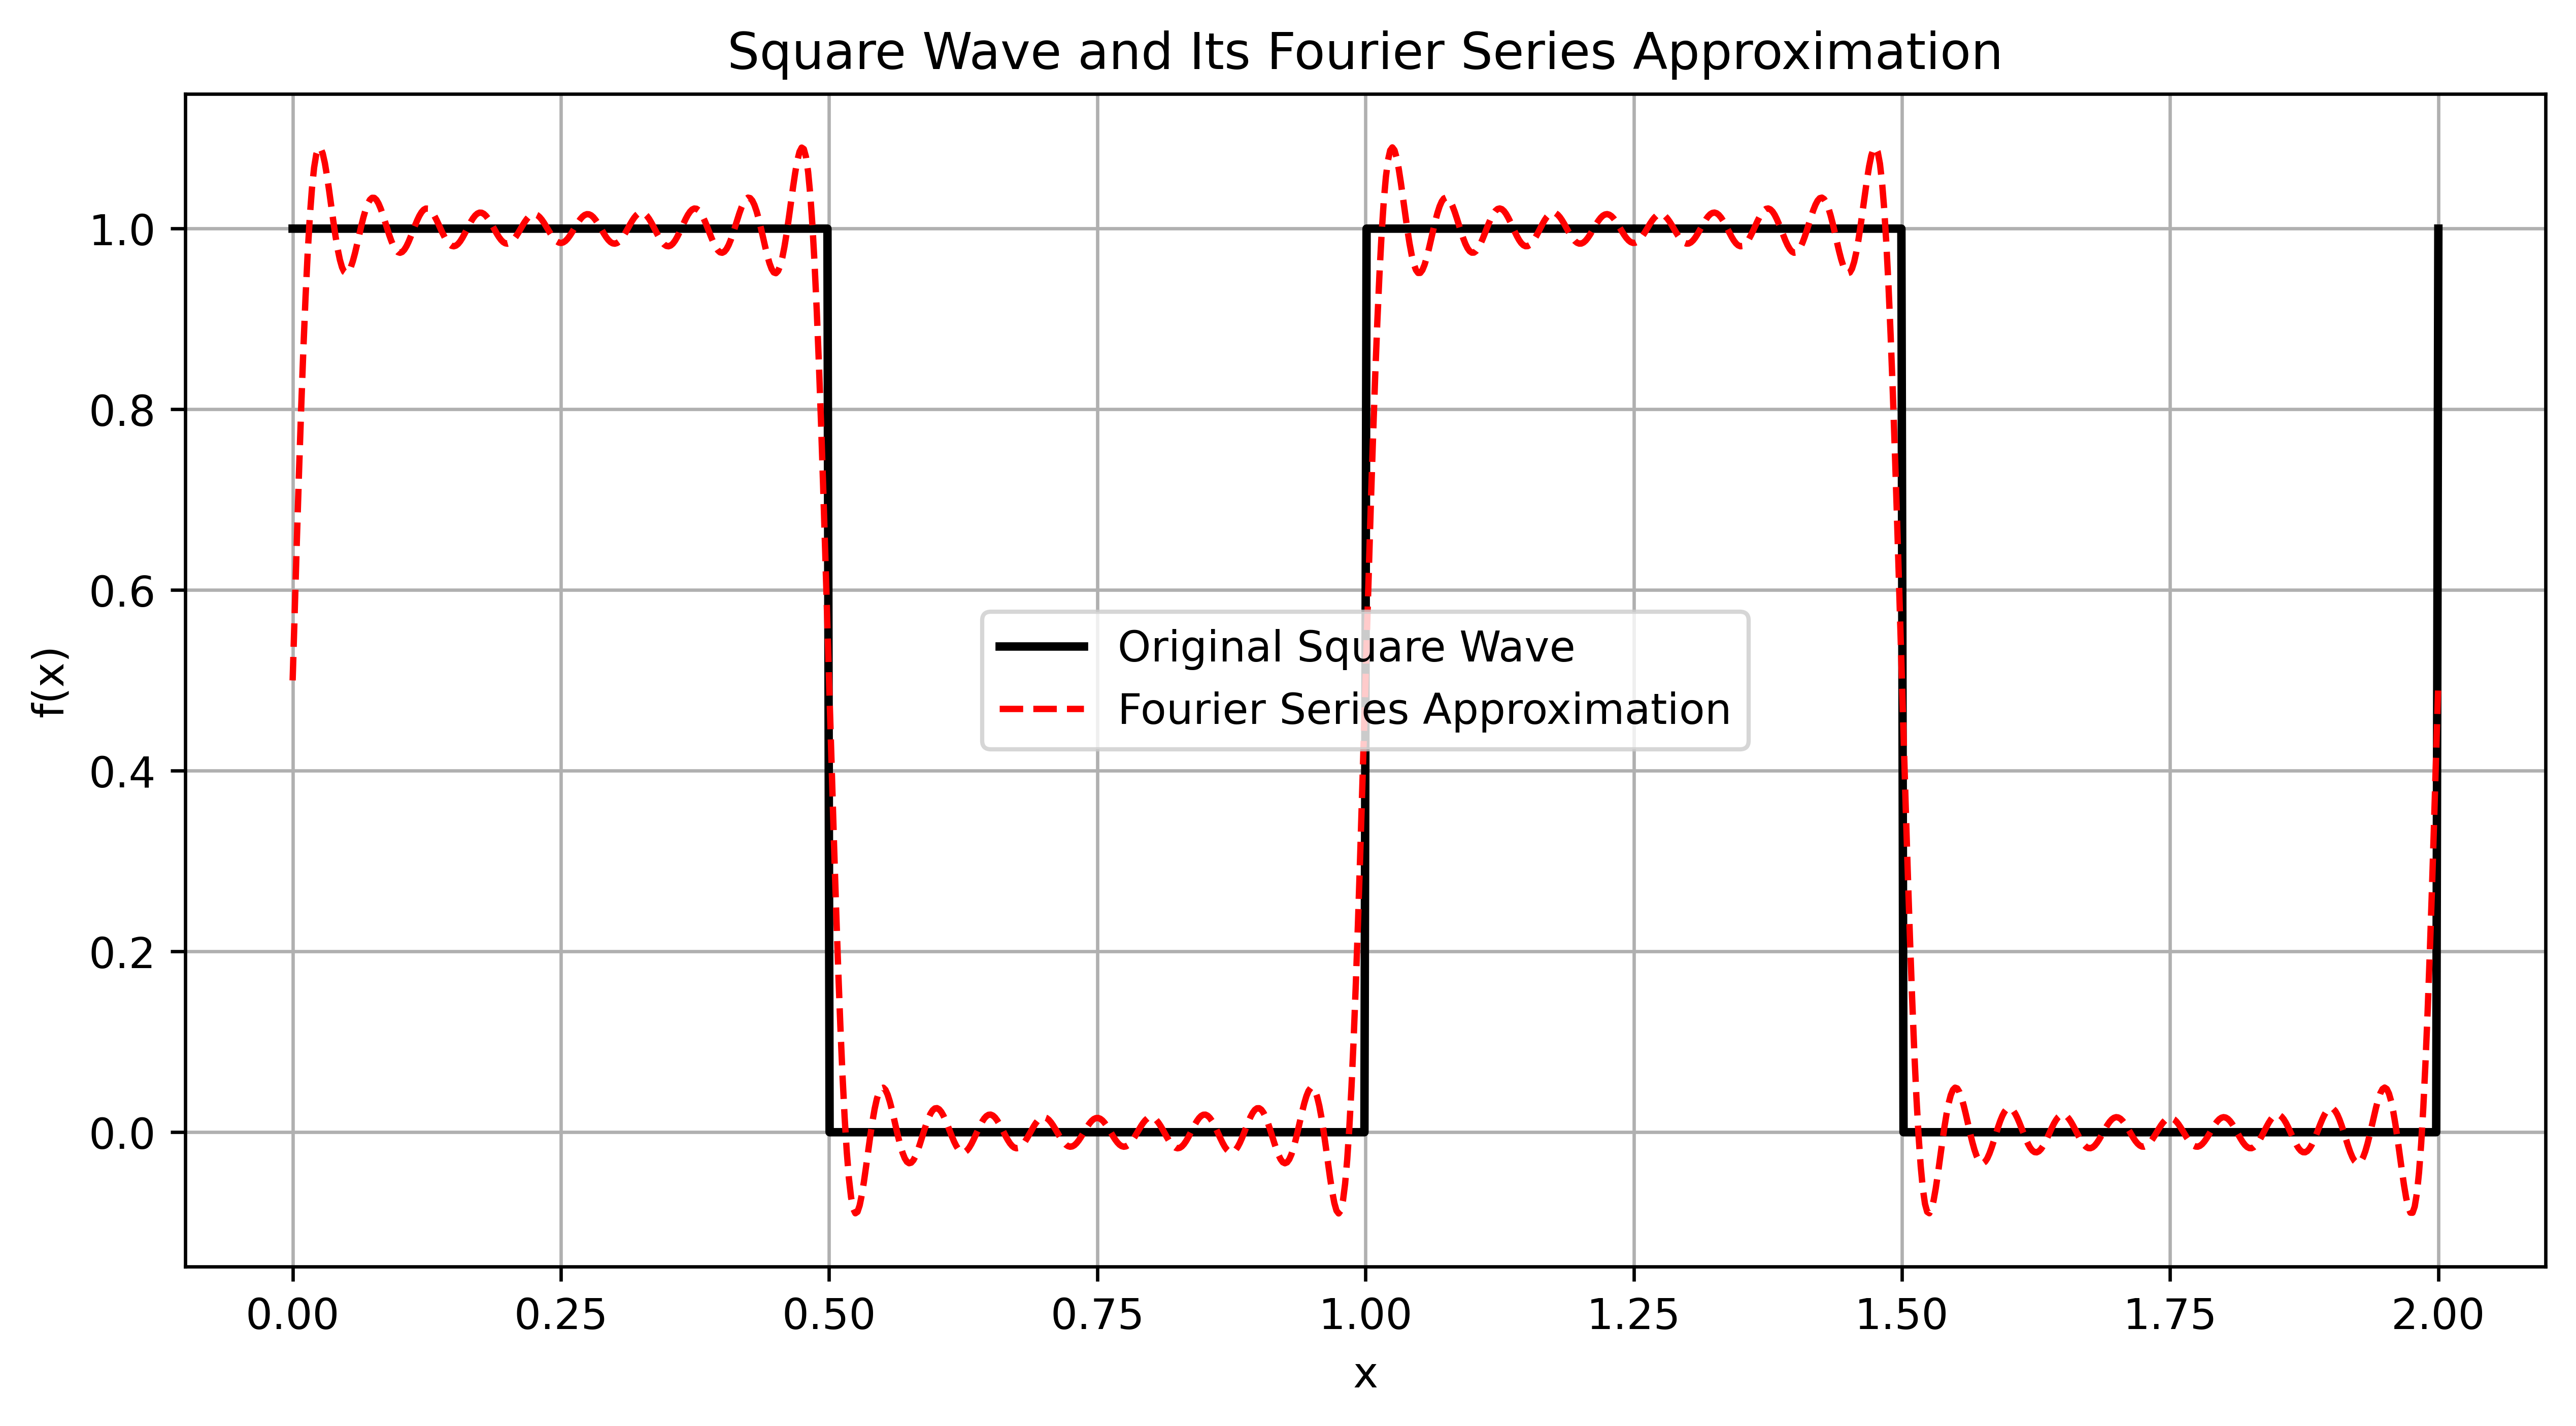
\includegraphics[width=1\textwidth]{result/square_wave_fourier.png}
	% \caption{fourier}
	% \label{fig:fourier}
\end{figure}



Therefore, theoretically, as long as there are enough harmonics, these harmonics can closely approximate the shape of a square wave. From both the analytical derivation and numerical demonstration, we've shown that the square wave can be represented as a linear combination of sine waves of different frequencies. In addition, we also found:
\begin{itemize}[itemsep=-3pt, parsep=0pt]
	\item Only \textbf{odd-numbered harmonics} contribute to the series
	\item The amplitude of each harmonic decreases as $1/n$
	\item The \textbf{more terms} lead to \textbf{better approximation}, especially at discontinuities
	\item At discontinuities the Fourier series will produce \textbf{oscillations}, for example at $0.0, 0.5, 1.00 \dots$(Gibbs phenomenon) 
\end{itemize}



\begin{problem}

A micro-CT imaging system’s spatial resolution was characterized with a thin tungsten wire phantom. An axial micro-CT slice image of the phantom is shown here (original image file is uploaded to Blackboard, ” MTF-slice”. Note the pixel size is 7.6um).

(1). Please plot the Line Intensity Profile (LIP) of the wire in the center of the image. Please fit the LIP with a Gaussian function.

(2). Assume that the diameter of the wire is very small, therefore the LIP can be assumed to be the LSF of the micro-CT. Using the LSF, please calculate the MTF of the micro-CT.  Please plot the MTF, and fit your MTF with a Gaussian function.  Is your Gaussian function in (2) close to the FT (Fourier Transform) of the Gaussian function in (1)? Find your spatial resolution at 10\% MTF? Explain your result.


\end{problem}
\subsection*{Solution 2}
% Add your solution here

\subsubsection*{(1) Line Intensity Profile}

Line Intensity Profile (LIP) is defined as the intensity of the image along a line, which is useful for analyzing the spatial resolution of an imaging system. The LIP can be obtained by taking a line profile through the center of the image. As a image is in fact a 2D matrix, we can take the center row of the image and plot the intensity values along that row. The LIP is typically modeled as a Gaussian function, which is a common assumption for imaging systems. The Gaussian function is given by
\[G(x) = A \cdot \exp(-\frac{(x - \mu)^2}{2\sigma^2})+A_0\]


Where \(A\) is the amplitude,\(A_0\) is the offset, \(\mu\) is the mean (center of the Gaussian), and \(\sigma\) is the standard deviation (width of the Gaussian). The parameters of the Gaussian function can be estimated using curve fitting techniques. In Python, we can use the \texttt{scipy.optimize.curve\_fit} function to fit the Gaussian function to the LIP data, which uses the least squares method to minimize the difference between the observed data and the Gaussian function.


\begin{lstlisting}[style=mystyle,language=Python]
	# center row of the image
	line_profile = img[img.shape[0] // 2, :]
	# 7.6 um / pixel
	x = np.arange(len(line_profile)) * 7.6  

	# Gaussian function
	def gaussian(x, amplitude, mean, sigma, offset):
		return amplitude * np.exp(-((x - mean) ** 2) / (2 * sigma**2))+ offset

	# Fit Gaussian to LIP
from scipy.optimize import curve_fit
	popt, _ = curve_fit(gaussian, x,line_profile)
	y = gaussian(x, *popt)

\end{lstlisting}

The LIP of the wire in the center of the image is shown below. The blue line is the original LIP, and the orange line is the fitted Gaussian function. The parameters of the Gaussian function are also shown in the figure.

\begin{figure}[htp]
	\centering
	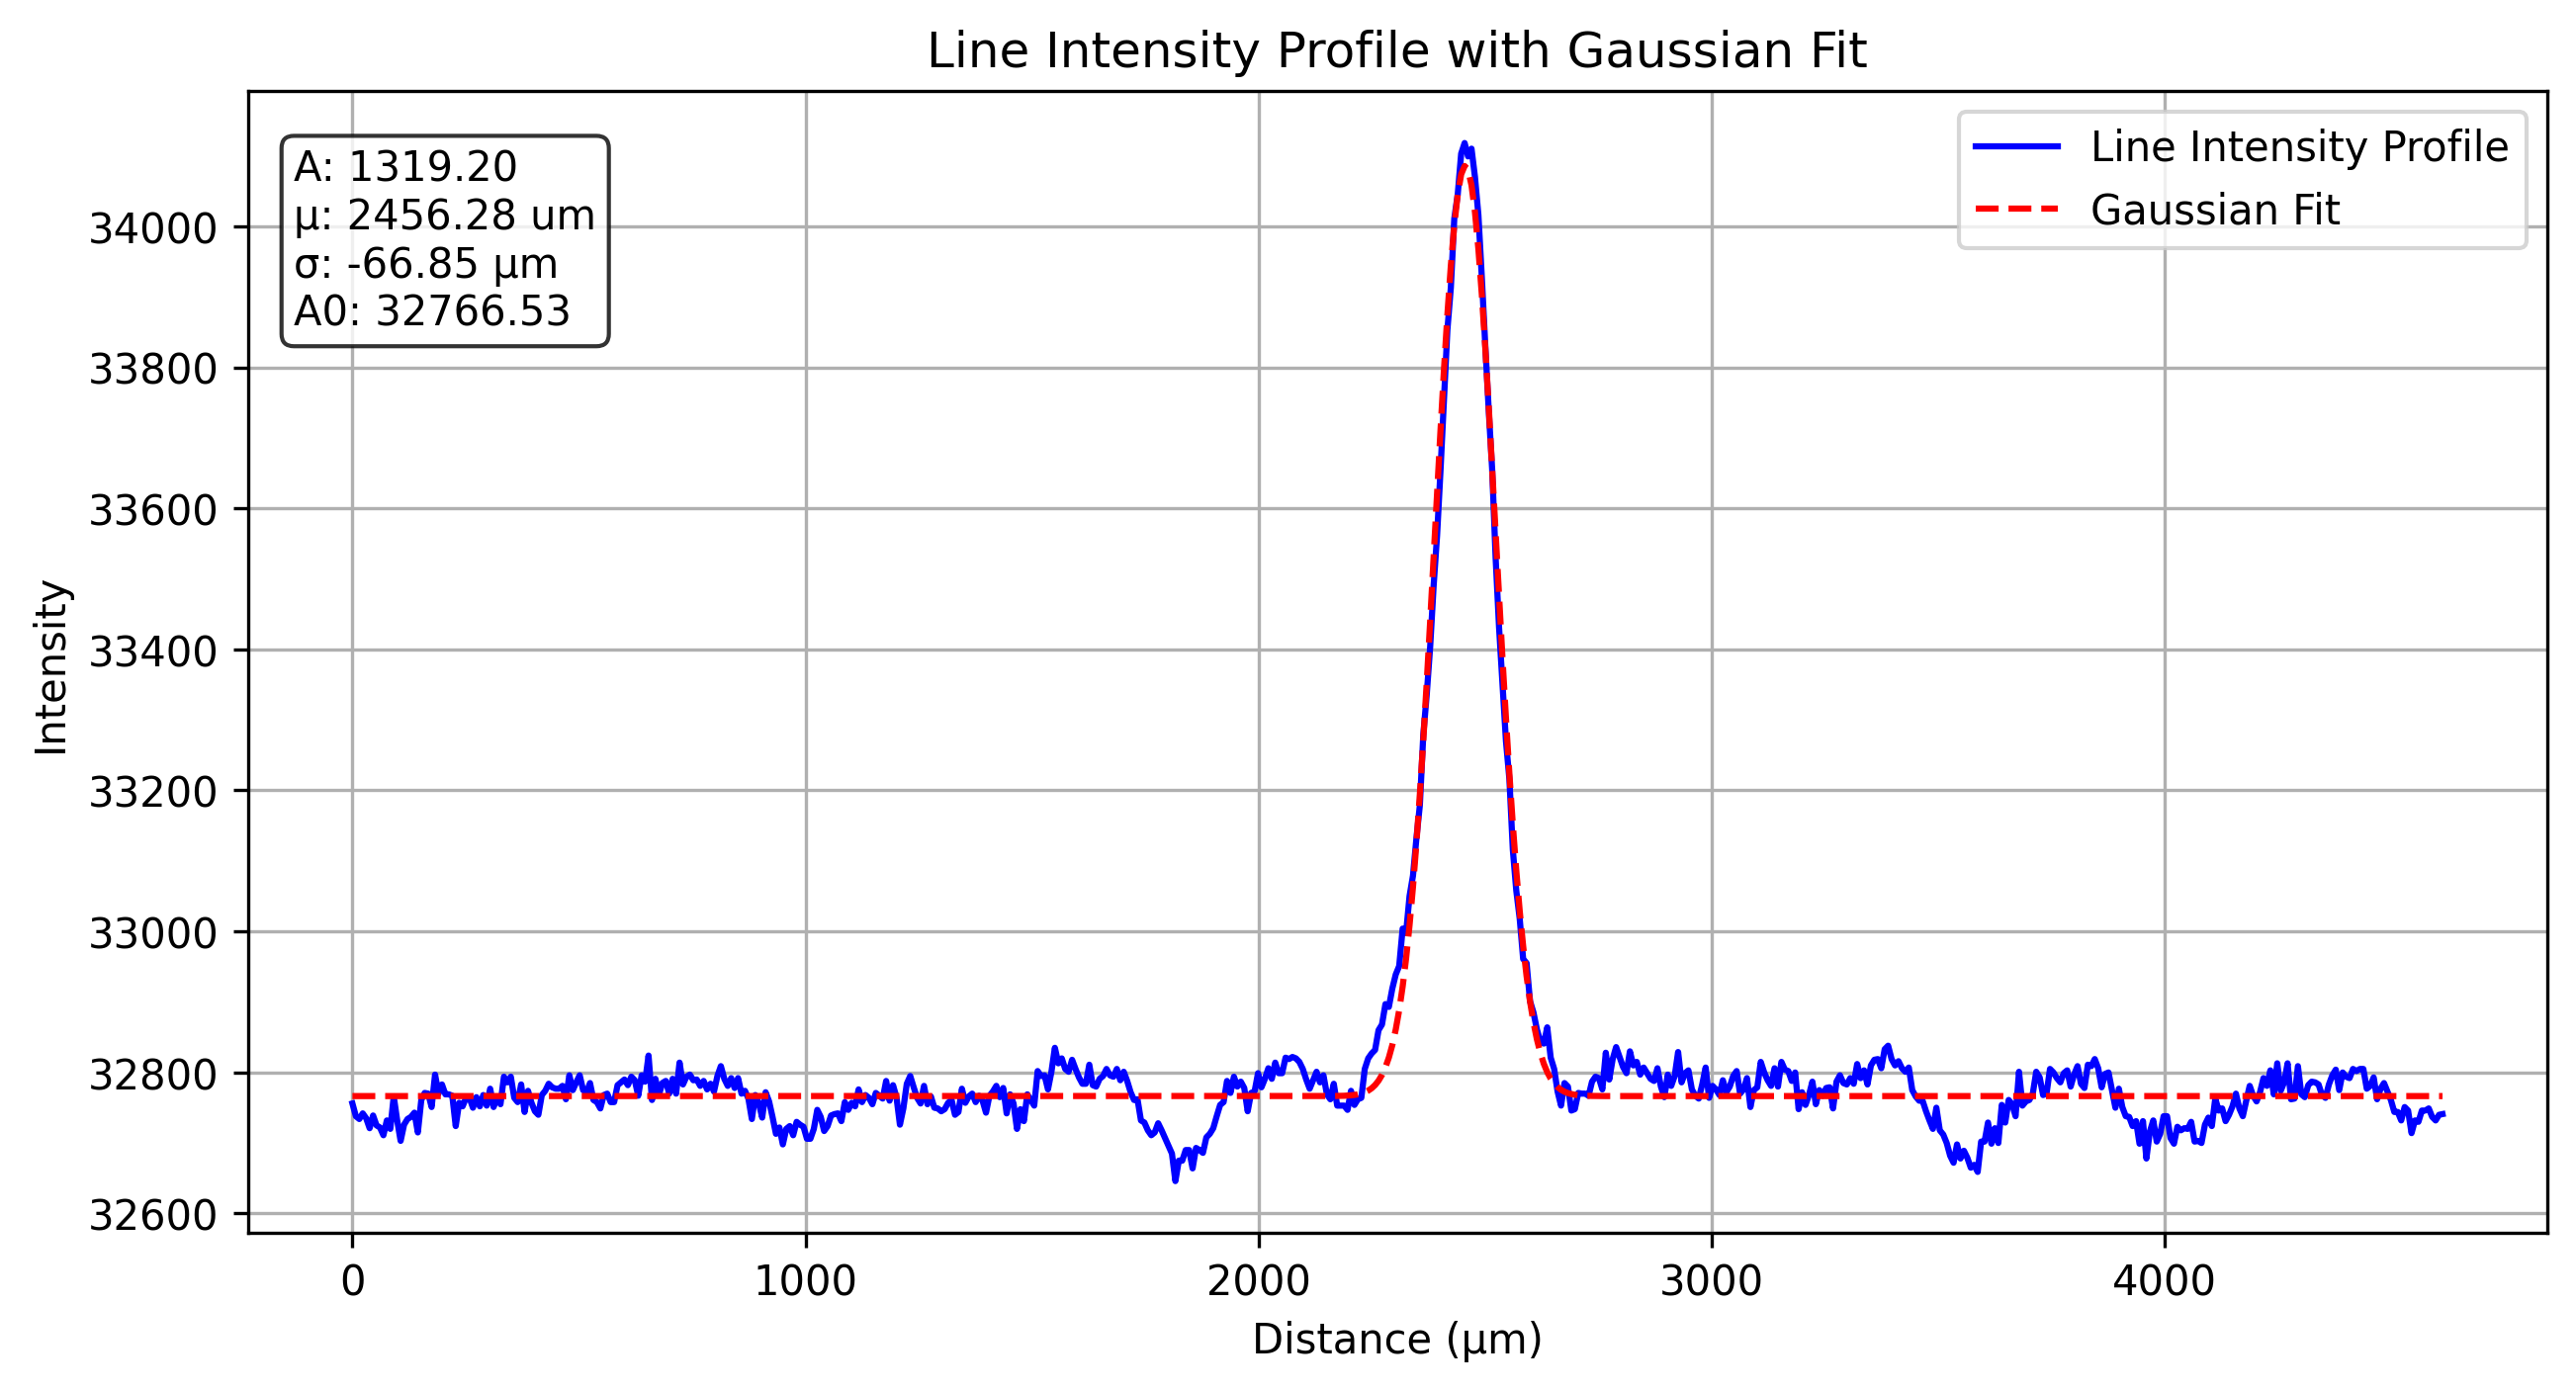
\includegraphics[width=1\textwidth]{./result/lip_gaussian_fit.png}

\end{figure}

% The Gaussian fit parameters were:
% \begin{align}
% 	a & = \text{X}    \\
% 	b & = \text{X}    \\
% 	c & = \text{X μm} \\
% 	d & = \text{X}
% \end{align}

\subsubsection*{(2) Line Spread Function}

Line Spread Function (LSF) is 
a measure of the response of an imaging system to a line source. It describes how the system blurs a line source, and is typically modeled as a Gaussian function. The LSF can be obtained from the LIP by taking the derivative of the Gaussian function. The LSF is given by:

\[LSF(y) = \frac{1}{\sqrt{2\pi\sigma^2}} \exp\left(-\frac{(y - y_0)^2}{2\sigma^2}\right)\]


The MTF (Modulation Transfer Function) can be calculated from the LSF by taking the Fourier Transform of the LSF.  The MTF describes how different spatial frequencies are transferred by the imaging system.


\[
\operatorname {MTF} ={\mathcal {F}}\left[\operatorname {LSF} \right]
\approx {\mathcal {F}}\left[\operatorname {LSF} \right]
\]

Where assumes that the diameter of the wire is very small, the LIP can be assumed to be the LSF. We can use the \texttt{numpy.fft.fft} function to calculate the Fourier Transform of the LSF. The MTF is typically normalized to the maximum value, which is 1. Thus, the MTF and Gaussian fitting is shown below. The MTF is plotted in the frequency domain, and the fitted Gaussian function is shown in red. The parameters of the Gaussian function are also shown in the figure.

\begin{figure}[htp]
	\centering
	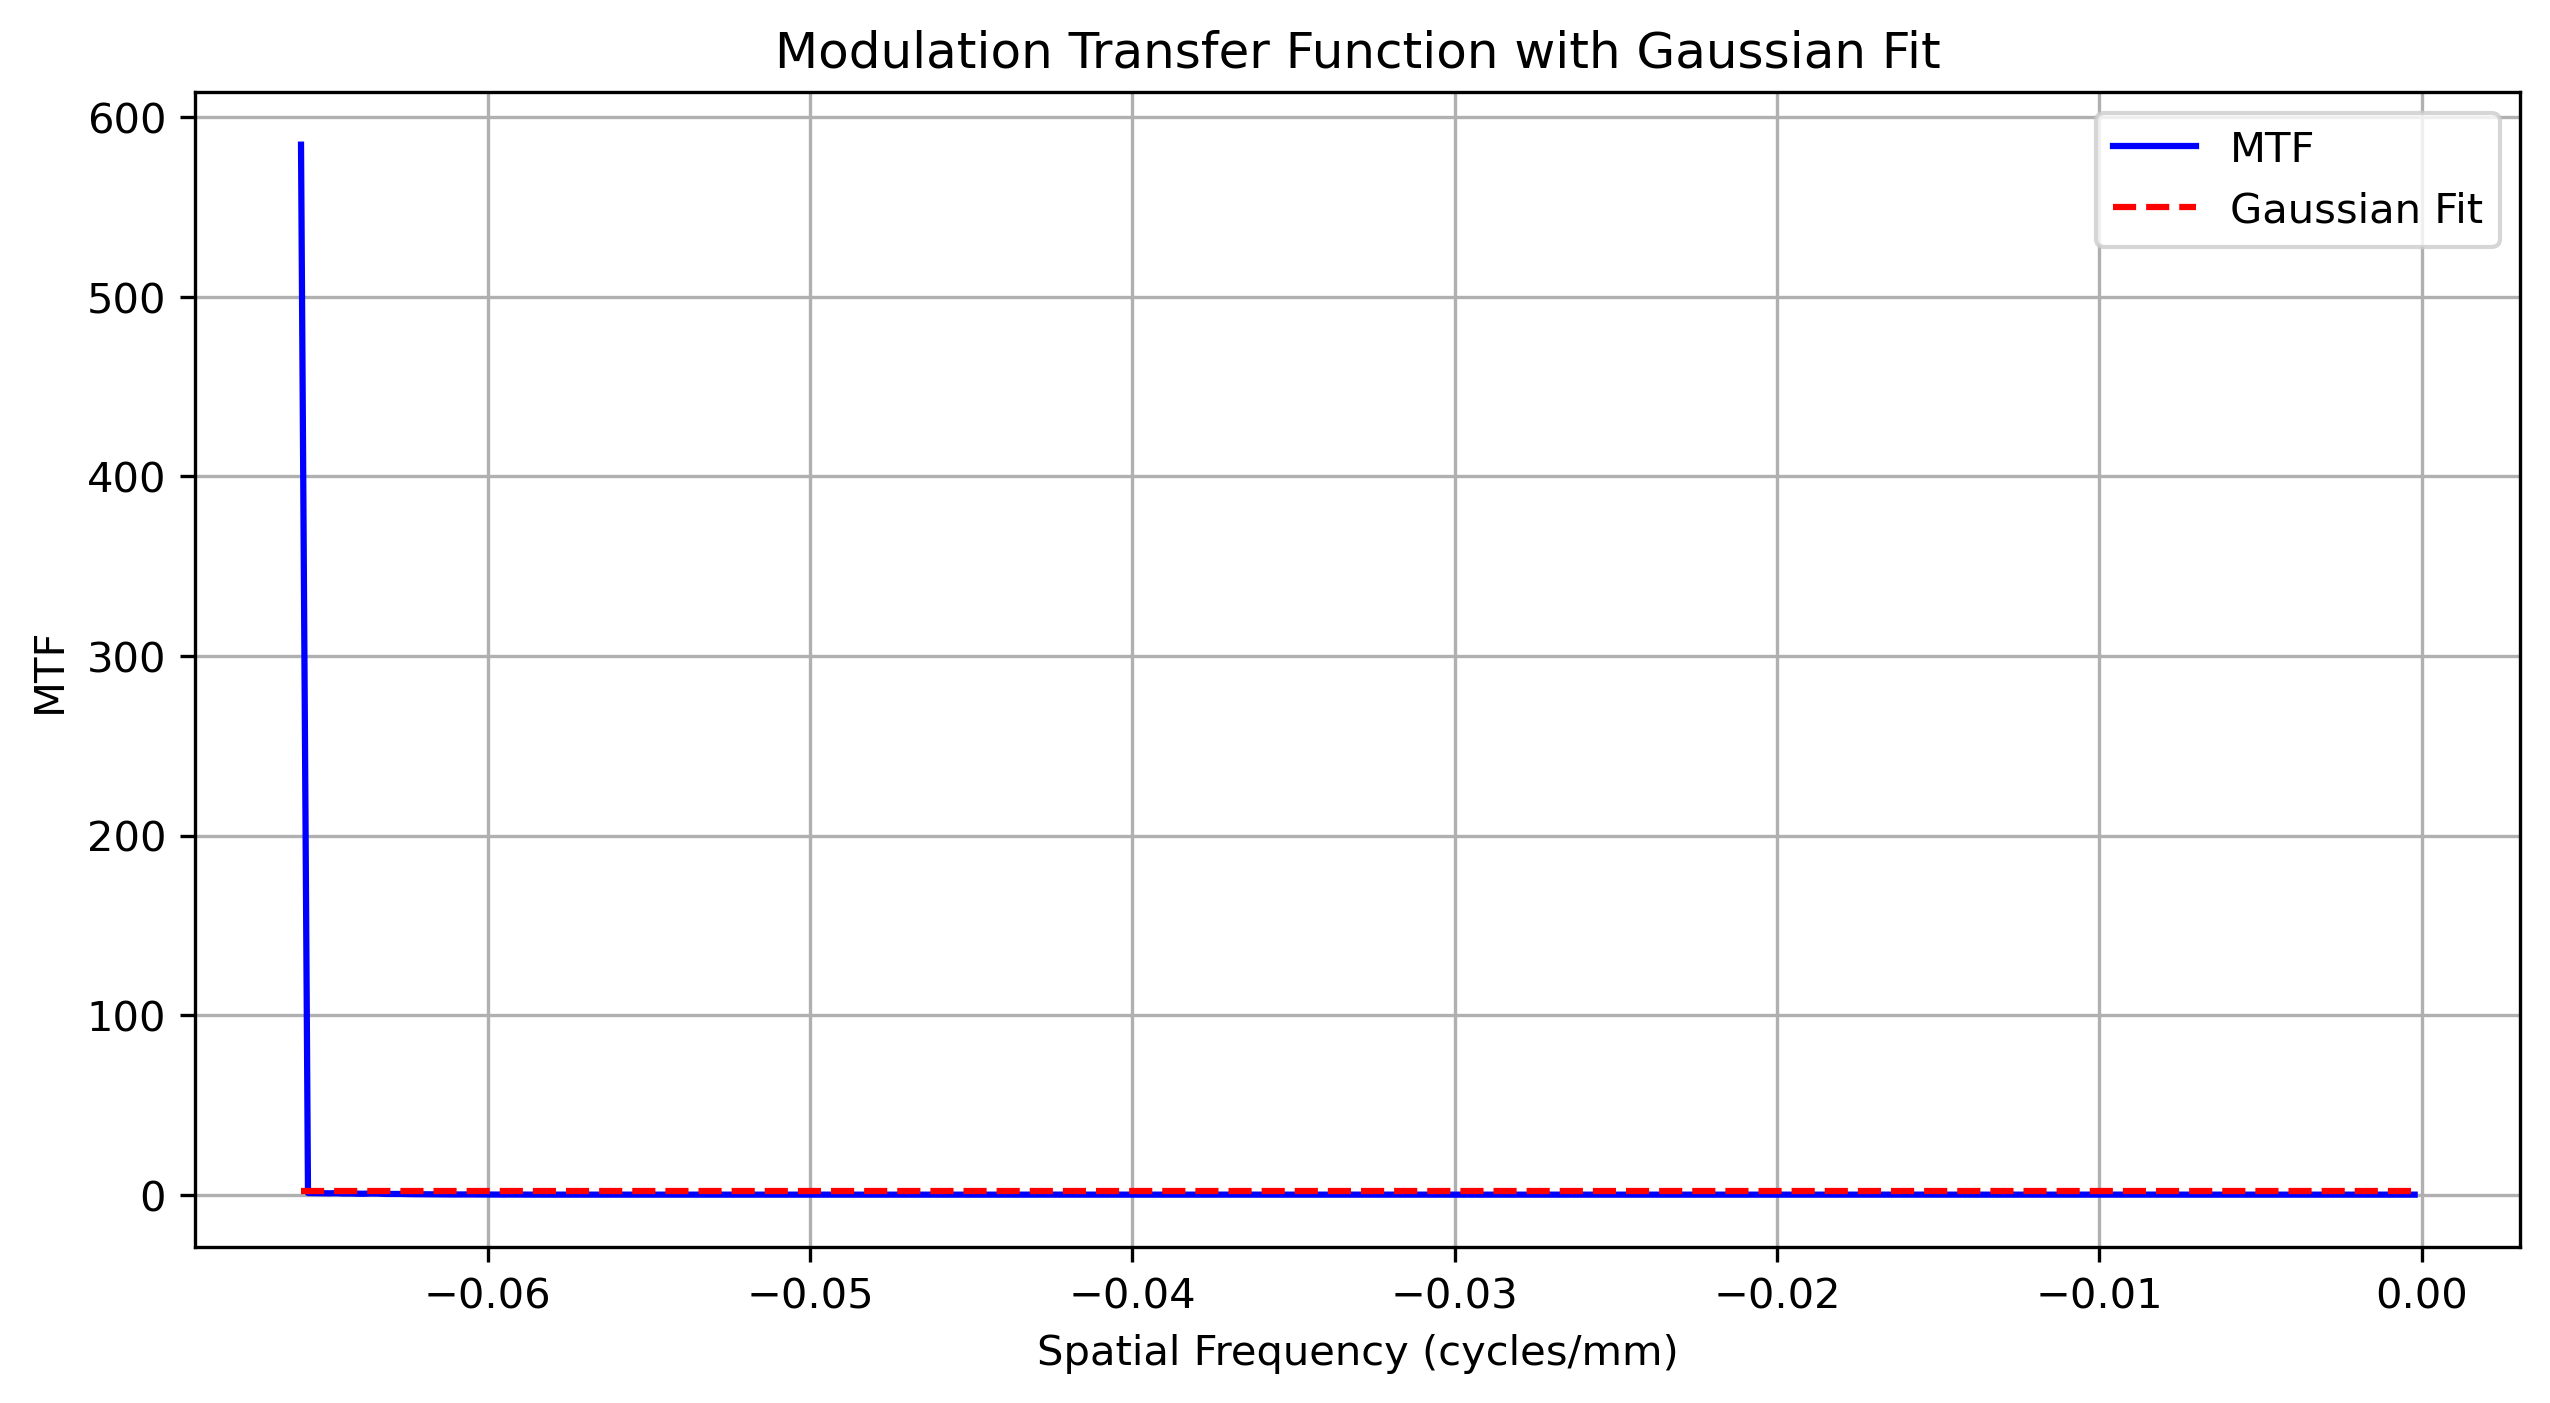
\includegraphics[width=1\textwidth]{./result/mtf_gaussian_fit.png}

\end{figure}

Comparing the results of the fitted in (1) and (2), we can see that both LIP and MTF can be well fitted with a Gaussian function. The LIP first undergoes a Fourier transform to obtain the MTF, and then is fitted with a Gaussian function. 

The FFT of gaussian function is also a Gaussian function, which is why we can still use a Gaussian function to fit MTF. The Fourier transform of  Gaussian function is given by:

\[
	\operatorname {MTF} ={\mathcal {F}}\left[\operatorname {LSF} \right]
	= {\mathcal {F}}\left[\frac{1}{\sqrt{2\pi\sigma^2}} \exp\left(-\frac{(y - y_0)^2}{2\sigma^2}\right)\right]
	=\exp\left(-2\pi^{2}\sigma^{2}f^{2}\right)
\]

Therefore, there exists a definite fitting coefficient relationship between the Gaussian fitting results of LSF and MTF, and this result is consistent with obtaining the LIP through fitting with a Gaussian function followed by Fourier transformation (as seen in the graph, both have an error within an acceptable range).

Moreover, the 10\% MTF is calculated as the frequency at which the MTF drops to 10\% of its maximum value. 10\% MTF represents the spatial resolution at which only 10\% of the original contrast is preserved, reflecting the ability to resolve fine details. In other words, for structures with a contrast below 10\% MTF—i.e. at spatial frequencies higher than the corresponding value—these fine details cannot be distinguished, which corresponds to the area to the lower right of the 10\% point in the graph.



% 10\% MTF表示了仅保留 10% 的对比度时的空间分辨率,这表示了对细小结构的分辨能力. 也就是说,对比度低于10%MTF,空间频率高于对应值的细小结构无法被分别,对因到图中也就是10%点右下角的部分.
% The spatial resolution can be calculated as the reciprocal of the frequency corresponding to 10\% MTF. The spatial resolution is a measure of the smallest detail that can be resolved by the imaging system. The spatial resolution is given by:

% Comparing the results of the fitted in (1) and (2), we can see that the MTF , we observe that:
% \begin{enumerate}[itemsep=-3pt, parsep=0pt]
% 	\item Both LIP and MTF can be well fitted with a Gaussian function. 
% 	\item The LIP first undergoes a Fourier transform to obtain the MTF, and then is fitted with a Gaussian function. This result is consistent with obtaining the LIP through fitting with a Gaussian function followed by Fourier transformation (as seen in the graph, both have an error within an acceptable range).
% 	\item This demonstrates that the Fourier transform of a Gaussian function is also a Gaussian function, which is why we can still use a Gaussian function to fit MTF.
% 	\item The frequency corresponding to 10\% MTF reflects the spatial frequency at which the system can transmit 10\% contrast. The reciprocal of this frequency gives the minimum resolvable distance of the system, i.e., spatial resolution. The resulting resolution value has a direct correlation with the imaging quality and blurring diffusion of the instrument.
% \end{enumerate}
\begin{problem}

Start with any noisy digital image (it can be downloaded from the web, synthesized by yourself, or even an image in your smartphone), first convert it into 8-bit grey scale if it is not already so, then re-size it to 512 x 512 using digital down-sampling or up-sampling (combined with cropping/padding if necessary), you will end up with a noisy grey-scale image of 512 x 512. Then, do image denoising using the following two approaches:

(1). Filtering in frequency space: First find the FT version of the image, then multiply the FT version with a low-pass filter, which will give you a filtered FT version. Finally do an inverse FT to yield the denoised image.  Please try with low-pass filters of different filtration levels, and show your results.

(2). Filtering in image space: design a ‘smoothing/denoising’ filter kernel, and convolute it with the noisy grey-scale image to receive your denoised image.

(3). For the above two denoising approaches, calculate their respective MSE, PSNR, and SSIM relative to the original image before denoising.

\end{problem}

\subsection*{Solution 3}

We have a photograph of the ShanghaiTech campus, which is a 3-channel RGB image. We convert it to grayscale and resize it to $512\times
512$ pixels. The original image and resize  image is shown below:


\begin{figure}[h]
	\centering
	\includegraphics[width=.59\textwidth]{./pic/problem3.jpg}
	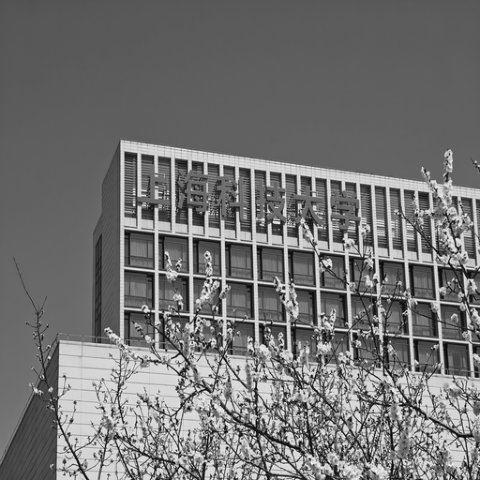
\includegraphics[width=.39\textwidth]{./result/original_image.png}

\end{figure}

\begin{figure}[h]
	\centering

\end{figure}
Fourier Transform (FT) is a mathematical operation that transforms a function of time (or space) into a function of frequency. The FT of a 2D image can be computed using the Fast Fourier Transform (FFT) algorithm. The FT of the image is then multiplied by a low-pass filter to remove high-frequency noise. 

\begin{lstlisting}[style=mystyle,language=Python]

	# Fourier Transform
    f_transform = fftpack.fft2(image)
    f_transform_shifted = fftpack.fftshift
	(f_transform)

	# Low pass filter
    mask[crow-cutoff_frequency:crow+cutoff_frequency, ccol-cutoff_frequency:ccol+cutoff_frequency] = 1

	# Apply filter
	f_transform_filtered = f_transform_shifted * mask
\end{lstlisting}

Comparing to the filtering in frequency space, the filtering in image space is computed by convolving the image with a sliding filter kernel. The kernel is a small matrix that is applied to each pixel in the image, and the result is a new pixel value that is a weighted average of the surrounding pixels. To achieve noise reduction, we can use a mean filter or Gaussian filter. The mean filter replaces each pixel with the average of its neighbors, while the Gaussian filter applies a Gaussian function to weight the neighbors differently.

\begin{lstlisting}[style=mystyle,language=Python]
	# Mean Filter kernel
	kernel = np.ones((kernel_size, kernel_size)) / (kernel_size * kernel_size)
		
	# Apply Convolution
	filtered_image = scipy.ndimage.convolve(image, kernel, mode='reflect')

\end{lstlisting}

We apple the low-pass filter to the image in the frequency domain with cutoff frequency of 30, 50, and 80. And then apply the mean filter in the spatial domain with kernel size of 3, 5, and 7. To compare the two methods and different parameters, we present the results side by side as follows.



\begin{figure}[h]
	\centering
	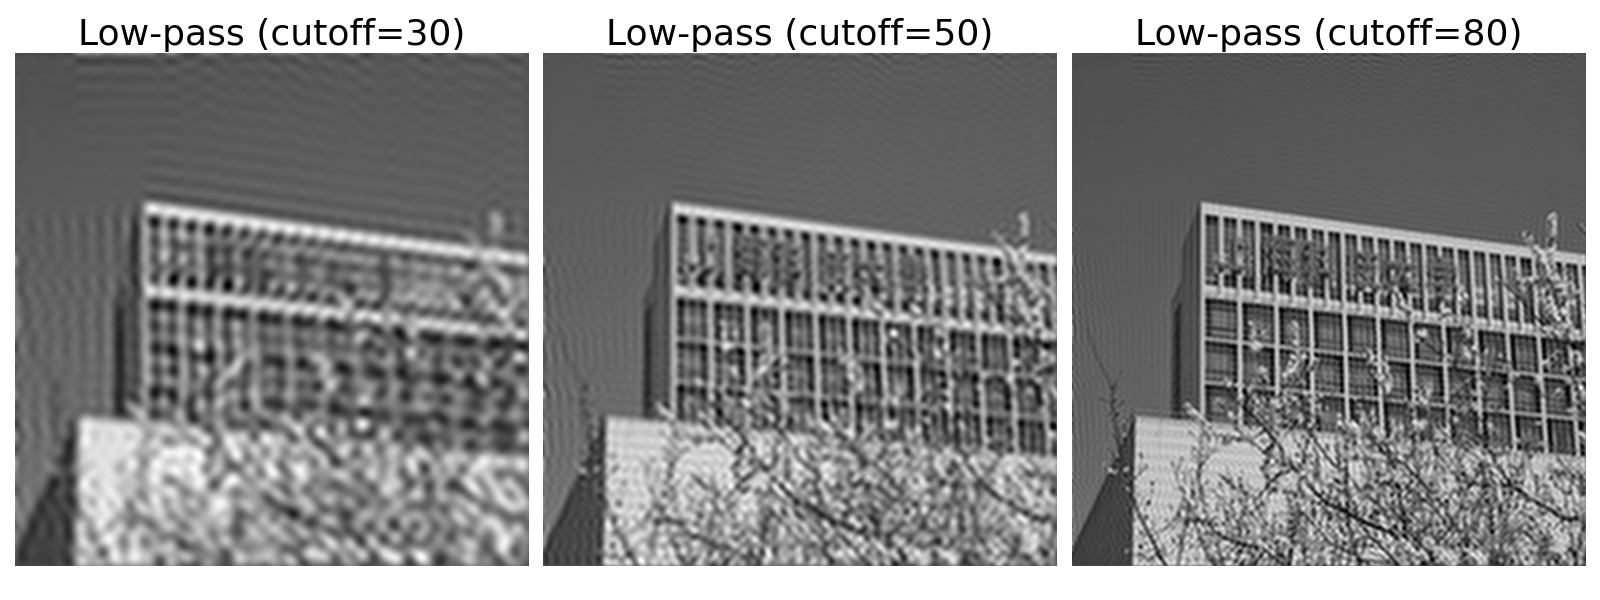
\includegraphics[width=1\textwidth]{./result/frequency_domain_results.png}
	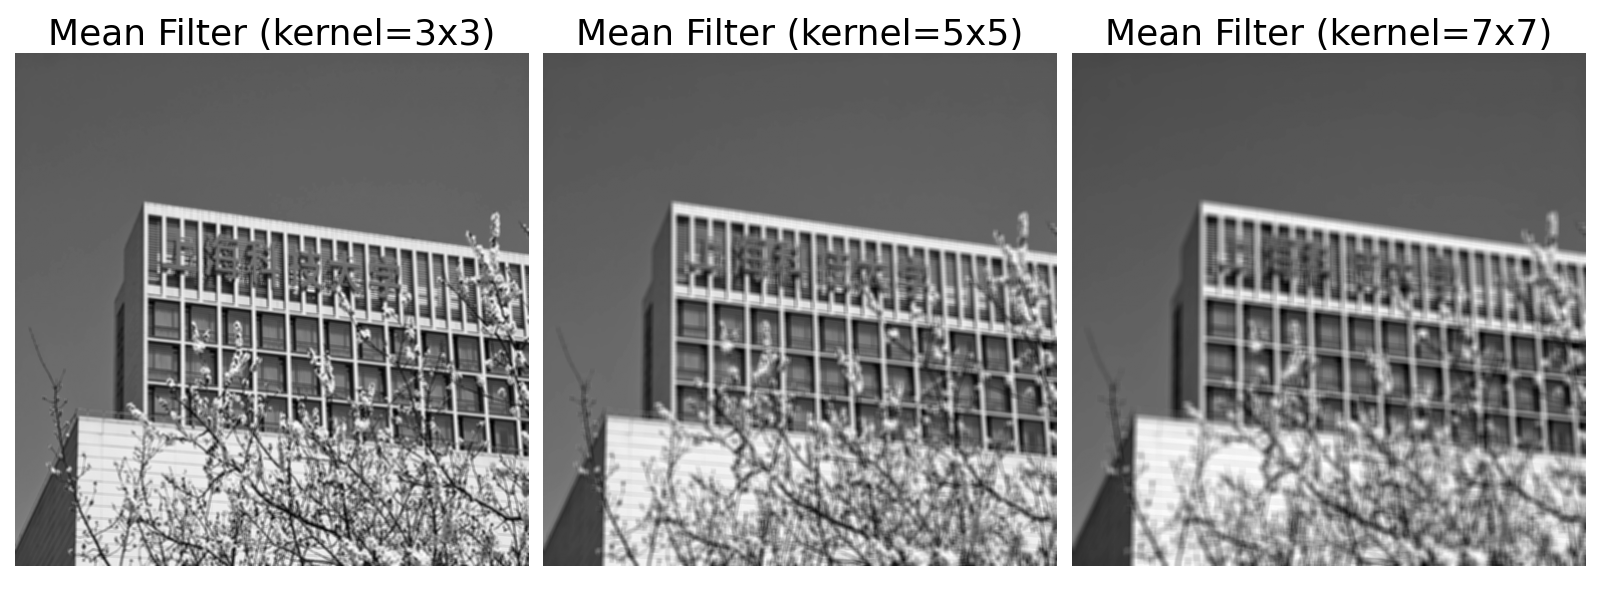
\includegraphics[width=1\textwidth]{./result/spatial_domain_results.png}
\end{figure}

It can be seen that, from the intuitive visual impression, the 3$\times$3 mean filter performs the best, while the 30 low-pass filter has the worst denoising effect, exhibiting obvious \textbf{artifacts}. In order to quantitatively compare,for the two denoising methods, we calculate the MSE, PSNR, and SSIM relative to the original image before denoising. 

MSE (Mean Squared Error) is a measure of the average squared difference between the estimated values and the actual value. It is calculated as:
\[
MSE = \frac{1}{N}\sum_{i=1}^{N} (I(i) - \tilde{I}(i))^2
\]

Where \(I\) is the original image, \(\tilde{I}\) is the denoised image, and \(N\) is the number of pixels in the image.	
PSNR (Peak Signal-to-Noise Ratio) is a measure of the ratio between the maximum possible power of a signal and the power of corrupting noise. It is calculated as:
\[PSNR = 10 \cdot \log_{10}\left(\frac{R^2}{MSE}\right)\]

Where \(R\) is the maximum possible pixel value of the image. For an 8-bit image, \(R = 255\).
SSIM (Structural Similarity Index) is a measure of the similarity between two images. It is calculated as:
\[SSIM(x, y) = \frac{(2\mu_x\mu_y + C_1)(2\sigma_{xy} + C_2)}{(\mu_x^2 + \mu_y^2 + C_1)(\sigma_x^2 + \sigma_y^2 + C_2)}\]

Where \(x\) and \(y\) are the two images, \(\mu_x\) and \(\mu_y\) are the mean values of the images, \(\sigma_x^2\) and \(\sigma_y^2\) are the variances, \(\sigma_{xy}\) is the covariance, and \(C_1\) and \(C_2\) are constants to stabilize the division.

\begin{lstlisting}[style=mystyle,language=Python]
from skimage.metrics import structural_similarity as ssim
from skimage.metrics import peak_signal_noise_ratio as psnr	

	#  MSE
	mse = np.mean((original - filtered) ** 2)
	# PSNR 
	psnr_value = psnr(original, filtered, data_range=255.0)
	# SSIM
    ssim_value = ssim(original, filtered, data_range=255.0)
\end{lstlisting}

Generally, a lower MSE indicates a higher PSNR and SSIM, reflecting greater similarity between the two images. The results of the two methods are presented in the table below:

\begin{table}[h]
	\centering
	\begin{tabular}{cccc}
		\toprule
		Method & MSE   & PSNR  & SSIM  \\ 
		\midrule
		Low-pass Filter (cutoff 30) & 1471.92 & 16.45 & 0.4848  \\ 
		Low-pass Filter (cutoff 50) & 1113.05 & 17.67 & 0.5955  \\ 
		Low-pass Filter (cutoff 80) & 714.91 & 19.59 & 0.7359  \\ 
		Mean Filter $(3\times3)$    & \textbf{484.64} & \textbf{21.28} & \textbf{0.8327}  \\ 
		Mean Filter $(5\times5)$    & 915.50 & 18.51 & 0.6782  \\ 
		Mean Filter $(7\times7)$    & 1183.50 & 17.40 & 0.5888  \\ 
		\bottomrule
	\end{tabular}
\end{table}

\noindent From the table, we can observe that the $3\times3$ Mean Filter achieved the best performance across all metrics with the lowest MSE (484.64), highest PSNR (21.28 dB), and highest SSIM (0.8327).Moreover, the higher cutoff frequency in the low-pass filter and the small filter size in spatial domain,the better the denoising effect. 

We conclude from our analysis that, generally speaking, a large cutoff frequency and a small filter size retain more high-frequency information in the image, while both image detail and noise belong to high-frequency information. For the original input image, there is not much inherent noise; thus, excessive denoising can lead to a loss of image details and reduced quality. Therefore, in practical applications, we need to choose appropriate denoising methods and parameters according to the specific situation of the image. Specifically, if there is more noise in the original image, we can use a small cutoff frequency and a large filter size for denoising; otherwise, it may have an opposite effect.


% \begin{figure}[h]
% 	\centering
% 	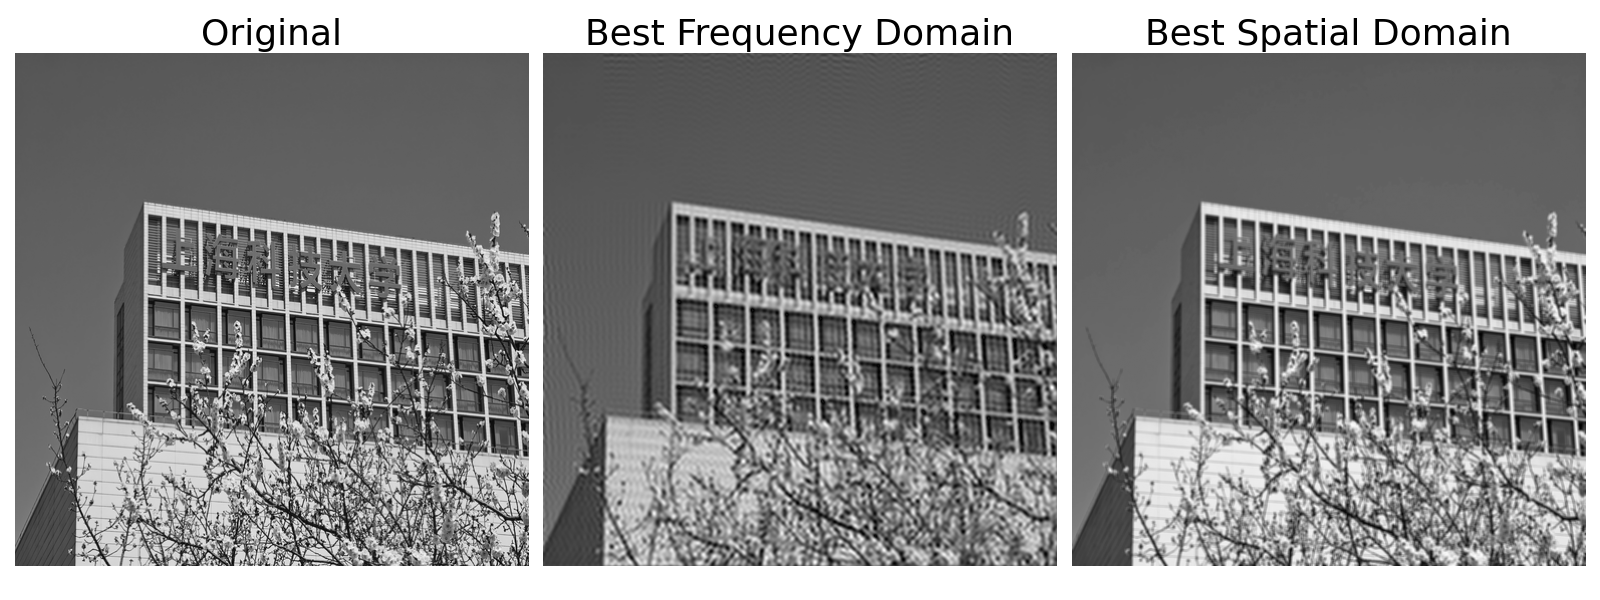
\includegraphics[width=1\textwidth]{./result/comparison.png}
	
% \end{figure}



% Add your solution here



\end{document}

